\documentclass[10pt,twocolumn,letterpaper]{article}

\usepackage{cvpr}
\usepackage{times}
\usepackage{epsfig}
\usepackage{graphicx}
\usepackage{amsmath}
\usepackage{caption}
\usepackage{subcaption}
\usepackage{booktabs}
\usepackage{amssymb}
%\usepackage{hyperref}

% Include other packages here, before hyperref.

% If you comment hyperref and then uncomment it, you should delete
% egpaper.aux before re-running latex.  (Or just hit 'q' on the first latex
% run, let it finish, and you should be clear).
\usepackage[breaklinks=true,bookmarks=false]{hyperref}

\cvprfinalcopy % *** Uncomment this line for the final submission

\def\cvprPaperID{****} % *** Enter the CVPR Paper ID here
\def\httilde{\mbox{\tt\raisebox{-.5ex}{\symbol{126}}}}

% Pages are numbered in submission mode, and unnumbered in camera-ready
%\ifcvprfinal\pagestyle{empty}\fi
%\setcounter{page}{4321}
\begin{document}

%%%%%%%%% TITLE
\title{Assignment 1: Predict diabetes via Perceptron}

\author{Moaz Mohamed\\
The University of Adelaide\\
Adelaide SA 5005\\
{\tt\small a1779177@student.adelaide.edu.au}
% For a paper whose authors are all at the same institution,
% omit the following lines up until the closing ``}''.
% Additional authors and addresses can be added with ``\and'',
% just like the second author.
% To save space, use either the email address or home page, not both

}

\maketitle
%\thispagestyle{empty}

%%%%%%%%% ABSTRACT
%\begin{abstract}
  % The ABSTRACT is to be in fully-justified italicized text, at the top
  % of the left-hand column, below the author and affiliation
  % information. Use the word ``Abstract'' as the title, in 12-point
  % Times, boldface type, centered relative to the column, initially
  % capitalized. The abstract is to be in 10-point, single-spaced type.
  % Leave two blank lines after the Abstract, then begin the main text.
 %  Look at previous CVPR abstracts to get a feel for style and length.
%\end{abstract}

%%%%%%%%% BODY TEXT
\section{Introduction}

Over the last few years, deep learning had a significant impact in the medical field. 
The application of numerous Deep learning algorithms have been implemented in different sector of the medical field. In this paper Perceptron algorithm will be explored and its performance will be investigated on classification task to predict diabetes on the provided dataset.In addition to a complete review of the Perceptron algorithm describing its strength and weakness. An alternative algorithm will be introduced and explored that can mitigate some of the inherit weakness of Perceptron. 
%-------------------------------------------------------------------------
\section{Methodology and Background}

\subsection{Perceptron}
The Perceptron algorithm was invented by Frank Rosenblatt at Cornell university. \cite{Rosenblatt1958} Perceptron is a supervised linear classifier. In binary classification the Perceptron will find a hyperplane that is able to separate the two classes assuming that the two classes are linearly separable.\cite{Murphy2017} \cite{Minsky1969} 

the idea behind the perceptron was inspired by the neurons in the brain work. hence a neuron will only fire at the signal reaches a certain threshold. in turn the perceptron emulates such mechanism.  

\begin{figure}[h!]
  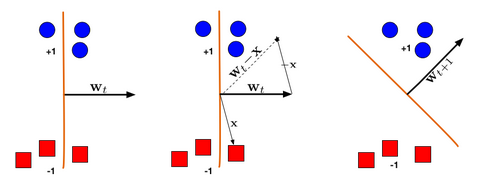
\includegraphics[width=\linewidth]{update.png}
  \caption{Perceptron update}
  \label{fig:Perceptron}
\end{figure}


The classification of a class depends on the data point location from the hyperplane. if its same direction as $\overrightarrow{w}$ or in opposite direction and a hyperplane is created that is Orthogonal to $\overrightarrow{w}$ hence the hyperplane becomes the decision boundary. the classification is characterized by the following equation $y_{i}\left( w_{i}^{T}x_{i}+b\right)$. assuming the binary outcomes are $(1, -1 )$ in both cases for the correct classification the previous terms should be $y_{i}\left( w_{i}^{T}x_{i}+b\right) \geq 0$. the idea behind the learning of a perceptron is to continuously update the $\overrightarrow{w}$ until all data points are correctly classified by $w_{i+1}=w_{i}+\eta \left( t_{i}-o_{i}\right) x_{i}$ as alluded to in figure \ref{fig:Perceptron}.

 
for easier implementation the bias term can be absorbed as such

\begin{equation}
\begin{bmatrix}
w \\
b
\end{bmatrix}^{T}\begin{bmatrix}
x_{i} \\
1
\end{bmatrix}
\end{equation}

which allows for a straight forward update for the perceptron. Gradient Descent can also be utilized in the original perceptron algorithm by allowing by having an linear activation function instead of unite step function(cite). 

\subsection{Support Vector Machines}

An alternative approach to pattern recognition is using Support Vector Machines(SVM). Which in hindsight very similar to the perceptron algorithm but SVM ensures finding a hyperplane taking into consideration the finding the hyperplane that can separate between the two classes with maximum margin. By finding the set of points $x_{j}$ to the boundary $\left| w^{t}x_{j}+w_{0}\right| =1$ hence the distance from the closet sample $x_{j}$ to $g(x)$ is 

\begin{equation}
\dfrac{\left| w^{t}x_{j}+w_{0}\right| }{\left\| w\right\| }=\dfrac{1}{\left\| w\right\| }
\end{equation}

where $g\left( x\right) =w^{t}x+w_{0}$

thus the margin is 

\begin{equation}
m=\dfrac{2}{\left\| w\right\| }
\end{equation}


which can be constructed as a quadratic function to 

minimize 
\begin{equation}
j\left( w\right) =\dfrac{1}{2}\times \left\| w\right\| ^{2}
\end{equation}

constraint to 
\begin{equation}
y_{j}\left( w^{T}x_{j}+w_{0}\right) \geq 1 , \forall j
\end{equation}

Such formulation does work on finding the optimal hyperplane and it can be solved with quadratic optimization tool such as CVXOPT OR MOSER. a slack variable can also be added to relax the SVM with $C$ as regularization parameter. 

minimization of 

\begin{equation}
\left\| w\right\| _{2}^{2}+c\times \dfrac{1}{n}\sum ^{n}_{j=1}\xi _{j}
\end{equation}

subject to 

\begin{equation}
\begin{aligned}y_{j}\left( w^{T}X_{j}+w_{0}\right) \geq 1-\xi j\\
\xi _{j}\geq 0,\forall n\end{aligned}
\end{equation}


Kuhn-Tucker theorem and Lagrange multipliers can be utilized to drive the previous problem from primal problem to dual problem. 

\begin{equation}
L_{D}\left( \alpha \right) =\sum ^{n}_{i}\alpha _{i}-\dfrac{1}{2}\sum ^{n}_{i=1}\sum ^{n}_{j=1}\alpha _{i}\alpha _{j}y_{i}y_{j} <X_{i}^{T}X_{j} >
\label{eqn:l}
\end{equation}

subject to 
\begin{equation}
\alpha _{j}\geq 0\forall j,\sum ^{n}_{j=1}\alpha _{j}y_{j}=0
\end{equation}

and the $\overrightarrow{w}$ and the bias term can be calculated as follows. 
\begin{equation}
W=\sum ^{n}_{j=1}\alpha _{j}y_{j}x_{j}
\label{eqn:weight}
\end{equation}

\begin{equation}
w_{0}=\dfrac{1}{y_{j}}-w^{T}x_{j}
\end{equation}
 
It is interesting to note that in equation \ref{eqn:weight} the weight vector can be formulated as summation of alpha, label and the support vector. instead of in the primal problem where the $\overrightarrow{w}$ is obtained directly from solving the quadratic optimization problem. Such difference allows for the usage for something called the "Kernel Trick".
 
\begin{equation}
L_{D}\left( \alpha \right) =\sum ^{n}_{j=1}\alpha _{j}-\dfrac{1}{2}\sum ^{n}_{i=1}\sum ^{n}_{j=1}\alpha _{i}\alpha _{j}y_{i}y_{j}K\left( x_{j},x_{i}\right) 
\label{eqn:lk}
\end{equation} 


\begin{figure}[h!]
  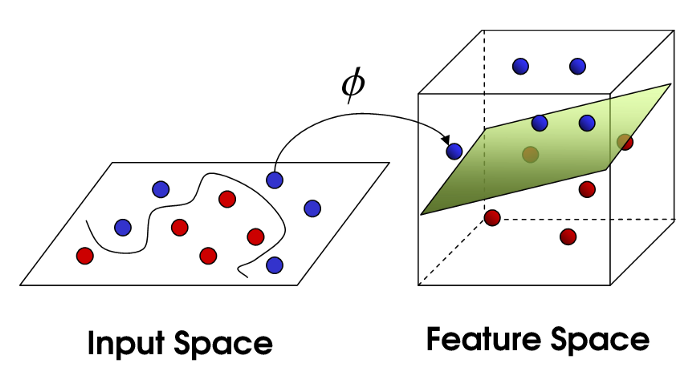
\includegraphics[width=\linewidth]{kernel.png}
  \caption{Mapping}
  \label{fig:kernel}
\end{figure}


\begin{equation}
K\left( x_{j},x_{i}\right) =\left( x_{i}^{T}x_{j}+1\right) ^{p}
\end{equation}


\begin{equation}
K\left( x_{i},x_{j}\right) =\exp \left( -\dfrac{1}{2\sigma ^{2}}\times \left\| x_{j}-x_{i}\right\| ^{2}\right) 
\end{equation}

the optimization problems for both equations \ref{eqn:lk} and \ref{eqn:l} except for the $( x_{j},x_{i})$ in equation \ref{eqn:lk} is being applied to a kernel and the data is being projected into higher dimensions. here the SVM is exploiting cover's theorem."A complex pattern-classification problem, cast in a high-dimensional space non-linearly, is more likely to be linearly separable than in a low-dimensional space, provided that the space is not densely populated." \cite{Cover1965} Which increases the complexity of the SVM by applying the kernel trick and enabling it to classify classes even in non-separable cases as demostrated in figure \ref{fig:kernel}

\section{Experimental Analysis.}
\subsection{Perceptron}

The perceptron algorithm does converge on hyperplane that  the two classes. but it doesn't converge on hyperplane that separate the two classes with the biggest margin between the two classes. in addition the algorithm inherit inability to classify class in non-linearly separable data as demonstrated in figure \ref{fig:percep_exp_non_lin} and \ref{fig:percep_exp_lin}. In-fact the algorithm will loop forever assuming no criteria for stoppage wasn't added.

%\begin{figure}[h!]
%  \centering
%  \begin{subfigure}[b]{0.2\textwidth}
%    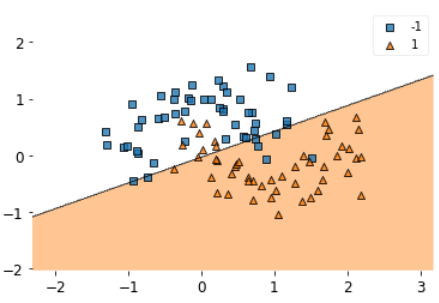
\includegraphics[width=\textwidth]{percep_non_lin.png}
%    \caption{Perceptron in linearly separable data}
%  \end{subfigure}
%  \begin{subfigure}[b]{0.2\textwidth}
%    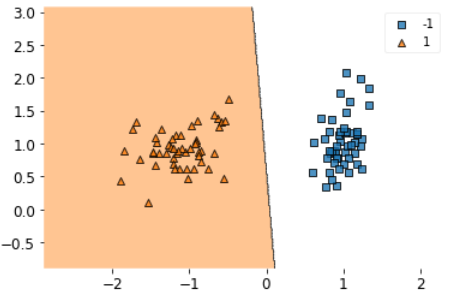
\includegraphics[width=\textwidth]{precep_lin.png}
%    \caption{Perceptron in non-linearly separable data}
%  \end{subfigure}
%  \caption{Perceptron decision boundary}
%  \label{fig:percep_exp}
%\end{figure}


\begin{figure}[h!]
  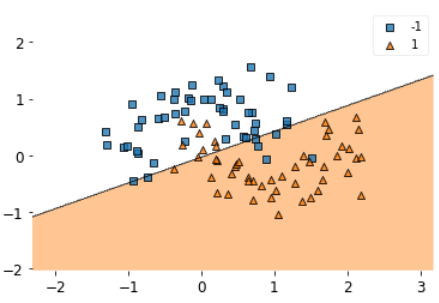
\includegraphics[width=\linewidth]{percep_non_lin.png}
  \caption{Perceptron decision boundary in linearly separable data}
  \label{fig:percep_exp_non_lin}
\end{figure}


\begin{figure}[h!]
  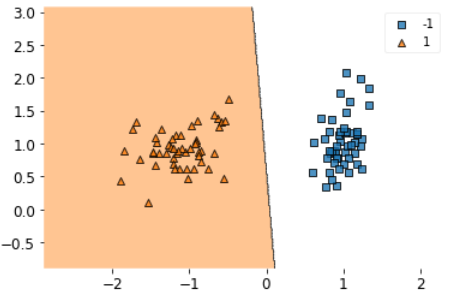
\includegraphics[width=\linewidth]{precep_lin.png}
  \caption{Perceptron decision boundary in non-linearly separable data}
  \label{fig:percep_exp_lin}
\end{figure}

\subsection{SVM Primal and Dual}
By utilizing the support vectors in eq \ref{eqn:weight} SVM is able to find the support vectors that can maximize the margin between the two classes as demonstrated in equation \ref{eqn:l} but SVM without utilizing a kernel SVM has the same weakness as Perceptron in that regard. But when a kernel is utilized and project the data into higher dimensions SVM is capable of finding a hyperplane between the two classes as demonstrated in figure \ref{fig:svm_exp_k}.

\begin{figure}[htb]
  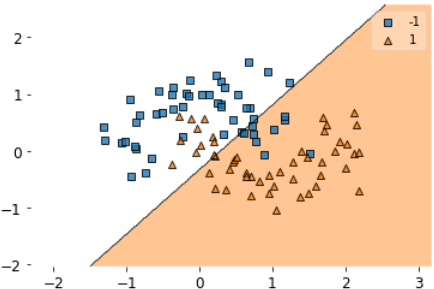
\includegraphics[width=\linewidth]{svm_lin_non_sep.png}
  \caption{SVM decision boundary in non-linearly separable data}
  \label{fig:svm_exp_non_lin}
\end{figure}

\vspace{3.00mm} 

\begin{figure}[htb]
  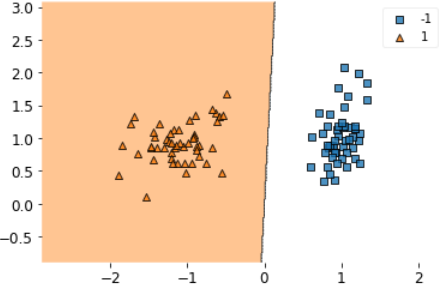
\includegraphics[width=\linewidth]{svm_lin_sep.png}
  \caption{SVM decision boundary in linearly separable data}
  \label{fig:svm_exp_lin}
\end{figure}

\vspace{50.00mm} 

\begin{figure}[htb]
  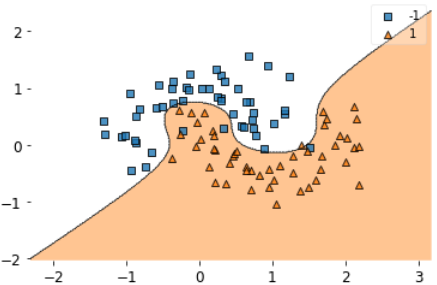
\includegraphics[width=\linewidth]{svm_k_non.png}
  \caption{SVM with polynomial kernel applied.Decision boundary in non-linearly separable data}
  \label{fig:svm_exp_k}
\end{figure}


\section{Performance on diabetes data-set}
In table \ref{tab:res} are the results. with aggressive hyper-parameter tuning all algorithms did perform with no apparent close contender. the diabetes dataset is full of missing values and noise with careful data cleaning steps i expect better results. 

\begin{table}[htb]
\centering
\begin{tabular}{|l|l|l|l|} 
\toprule
Algorithm         & Accuracy & precision & F1    \\ 
\hline
Perceptron        & 72\%     & 60\%      & 57\%  \\ 
\hline
SVM               & 73\%     & 63\%      & 58\%  \\ 
\hline
SVM + Polynomial  & 72\%     & 62\%      & 57\%  \\ 
\hline
SVM + Gaussian    & 71\%     & 58\%      & 58\%  \\
\bottomrule
\end{tabular}
\caption{Results}
\label{tab:res}
\end{table}

\section{Conclusion}
Perceptron and different variations of Support vector machines algorithm have been explored and analyzed. mathematical formulation of all the algorithms have been studied. decision boundaries for have been made for a careful study of the behavior of various algorithms in different data situations. Advantageous and weakness have been identified for all the explored algorithms. Perceptron and its creator have created and paved the way for the emergence of the field of machine learning. all subsequent algorithms builds on top of the weakness of the previous work as seen in perceptron, SVM and later kernalised SVM.
\section{Code}

all the code for this assignment is provided in this GitHub repo 
\url{https://github.com/RoastedKernel/uni_Machine_Learning}
\bibliography{egbib.bib} 
\bibliographystyle{ieeetr}

\end{document}
